% !TeX root = ./00_wrapper.tex
\documentclass[11pt, a4paper]{report}

% custom margins, required by UniTN
\usepackage[a4paper, left=2cm, right=2cm, top=2cm, bottom=2cm, footskip=1cm]{geometry}

% english document
\usepackage[utf8]{inputenc}
\usepackage[american]{babel}

% bibliography (see https://tex.stackexchange.com/questions/58152/how-to-emulate-the-traditional-bibtex-styles-plain-abbrv-unsrt-alpha-as-clo)
\usepackage{csquotes}
\usepackage[style=trad-plain]{biblatex}
\addbibresource{references.bib}

% fix urls in bibliography
\usepackage[hidelinks]{hyperref}
\renewcommand{\UrlFont}{\small\tt}

% units and nice numbers
\usepackage[group-separator={,}]{siunitx}

% images
\usepackage{graphicx}
\usepackage{subcaption}
\usepackage{float}

% tables
\usepackage{booktabs}

% footnotes: stick at bottom and do not reset counts between chapters
\usepackage[bottom]{footmisc}
\usepackage{chngcntr}
\counterwithout{footnote}{chapter}

% special symbols, eg. <, >
\usepackage{textcomp}

% pseudo code (NB: to load BEFORE cleveref)
\usepackage{setspace}
\usepackage[algoruled]{algorithm2e}

% cref command
\usepackage[noabbrev,capitalise]{cleveref}

% custom spacings
\usepackage{setspace}

% TODO: use only for draft versions
% \renewcommand{\baselinestretch}{1.5}

% list of acronyms
\RequirePackage[index=true]{acro}
\NewDocumentCommand\acrodef{mO{#1}mG{}}{\DeclareAcronym{#1}{short={#2}, long={#3}, #4}}
\NewDocumentCommand\acused{m}{\acuse{#1}}
\acrodef{PoW}{Proof-of-Work}
\acrodef{CPU}{central processing unit}
\acrodef{GPU}{graphics processing unit}
\acrodef{BGP}{Border Gateway Protocol}
\acrodef{ISP}{Internet Service Provider}
\acrodef{AS}{autonomous systems}
\acrodef{DNS}{Domain Name System}

% TODO: remove DRAFT and change date
\title{[DRAFT]\\Simulating large scale network attacks against Bitcoin}
\author{Davide Pedranz}
\date{\today}

\begin{document}

% TODO: remove this!
\begin{titlepage}
	\maketitle
\end{titlepage}

% TODO: set good margins for real print!
\begin{titlepage}

	% custom layout
	\pagestyle{empty}
	\newgeometry{top=0cm, bottom=0cm}

	% center the page vertically
	\vspace*{\fill}

	% center the page horizontally
	\begin{center}

		% university
		\vspace{-0.2cm}
		{
			\bfseries
			\Large {\huge U}NIVERSITY OF {\huge T}RENTO
		}

		% department
		\vspace{0.3cm}
		{\Large Department of Information Engineering and Computer Science}

		% logo
		\vspace{0.6cm}
		\begin{center}
			
\includegraphics[width=0.32\textwidth]{figures/unitn}
		\end{center}
		\vspace{0.6cm}

		% degree
		{
			\bfseries
			\Large Master's Degree in Computer Science
		}
		\vspace{0.3cm}
		\line(1,0){338}
		\vspace{0.3cm}

		% thesis
		{
			\Large Final Dissertation
		}

		% title
		\vspace{2cm}
		{
			\begin{spacing}{0.9}
				\huge \textsc{Simulating large scale network attacks against Bitcoin}
			\end{spacing}
		}
		\vspace{2cm}

		% advisor + student
		\Large
		\begin{center}
			\begin{tabular}{ccc}
				{\bfseries Advisor} & \hspace{5cm} {\bfseries Student} \\
				Alberto Montresor   & \hspace{5cm} Davide Pedranz      \\
			\end{tabular}
		\end{center}

		% year
		\vspace{3cm}
		{
			\bfseries
			\large Academic Year 2017-2018
		}

	\end{center}

	% center the page vertically
	\vfill

	% cleanup the custom layout
	\restoregeometry

\end{titlepage}


\tableofcontents
\listoffigures
\listoftables

\chapter{Bitcoin}
\label{chapter:bitcoin}
Bitcoin (BTC) is a decentralized digital currency without a central bank or single administrator.
The original paper \cite{bitcoin_2009} and the first implementation of Bitcoin were published respectively in November \num{2008} and January \num{2009} by an unknown person or group of people using the name of Satoshi Nakamoto \cite{bitcoin_website}.
Since its release, Bitcoin has gained popularity and attention of the media, especially between the end of \num{2017} and the beginning of \num{2018} \cite{bbc_2018, telegraph_2018, ilsole24ore_2018}.
Nowadays, Bitcoin is the most used and valuable cryptocurrency available on the market, with a price of over \SI{8000}{\$ \per BTC} and a market cap of about \num{141} billion \$ \cite{bitcoin_usage_study_2017, stats_coinmarketcap, stats_coinranking, stats_cryptocompare, stats_coincheckup, stats_moonstats}.
Bitcoin can be used for both online and in-shop payments, fast and low-cost money transfer, and pseudonymous money spending.

\bigskip
Bitcoin is a complex technology that takes advantage of modern cryptography and distributed algorithms to solve the complex Byzantine Consensus problem \cite{byzantin_generals_1982}.
This section covers the main building blocks and concepts and gives an overview of the overall working of Bitcoin.

\section{Blockchain}
The blockchain is a decentralized, distributed, public digital ledger that records Bitcoin transactions.
It is implemented as a chain of blocks, connected to each other using linked timestamping \cite{bitcoin_book_narayanan_2016, hash_function_wikipedia}:
each block stores the cryptographic hash of the previous one (\cref{fig:blockchain}).
This technique guarantees that the transactions stored in the ledger can not be changed easily, since a single modification would break the hashes of each following block in the chain.
The first block is called ``genesis'' and it is hard-coded in the software implementation.

Nodes that participate in the Bitcoin protocol run a consensus algorithm to agree on the order of blocks in the ledger:
in particular, it is enough to agree on the last block in the chain, thanks to the guarantees given by the linked timestamps.
The blockchain is stored in each computer that participates in the consensus:
the geographical distribution of nodes around the world and the decentralization of the protocol make attacks that try to change the history of transactions stored in the ledger very difficult or nearly impossible to achieve.

\begin{figure}[h]
	\centering
	\vspace*{0.25cm}
	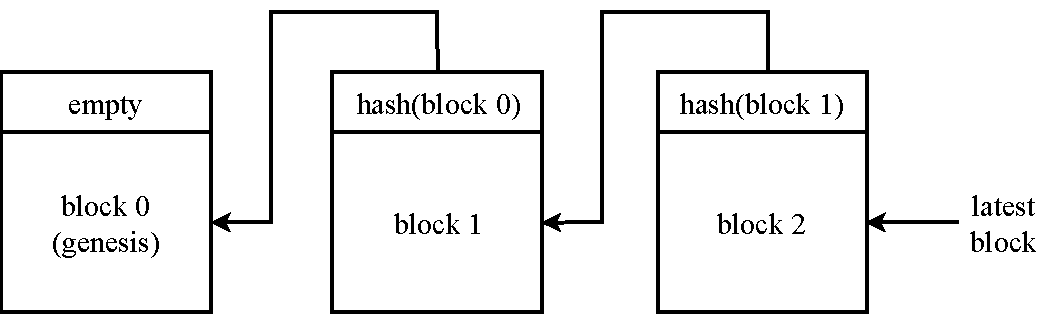
\includegraphics[scale=0.7]{figures/blockchain}
	\vspace*{0.25cm}
	\caption[Schematic representation of a blockchain.]{
		Schematic representation of a blockchain.
		A blockchain is a list of blocks, connected to each other with an hash pointer.
		Each block contains a set of transactions.
	}
	\label{fig:blockchain}
\end{figure}

\section{Blocks}
Each block contains about \num{3000} transactions.
By design, a new block is generated and appended to the blockchain every \SI{10}{minutes} on average \cite{bitcoin_2009}.
Bitcoin blocks are distributed using a peer-to-peer protocol, which is explained in detail in \cref{chapter:protocol}.

The transactions inside each block are organized as a Merkle tree \cite{merkle_tree_1980}, a special binary tree with hash pointers (\cref{fig:merkle}).
The items in the tree are grouped in pairs and the hash of each of them is stored in the parent node.
The parent nodes are then grouped in other pairs and their hashes are stored in their parents:
this construction is repeated recursively until a single root node is created.
In the specific case of Bitcoin, each item in the tree represents a single transaction.

\begin{figure}[h]
	\centering
	\vspace*{0.1cm}
	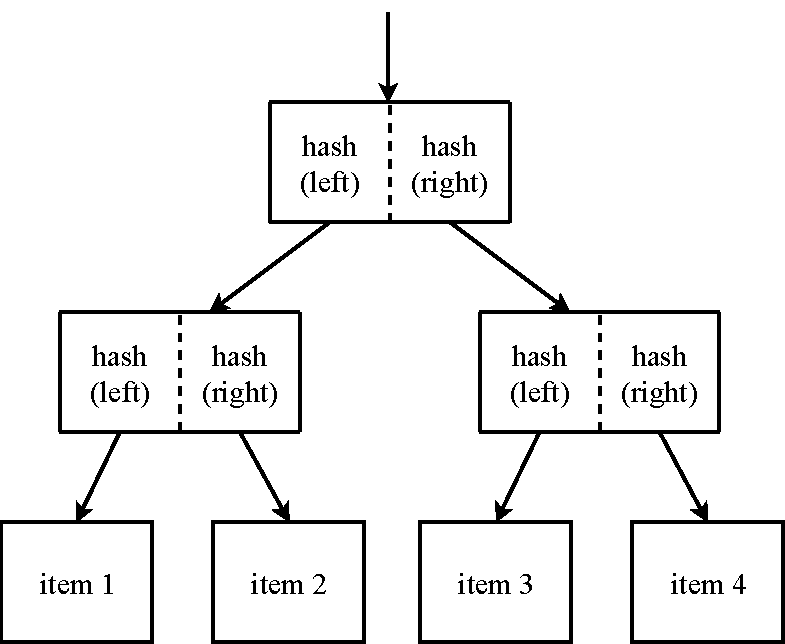
\includegraphics[scale=0.7]{figures/merkle}
	\vspace*{0.25cm}
	\caption{Schematic representation of a Merkle tree with \num{4} items.}
	\label{fig:merkle}
\end{figure}

The main advantage of using a Merkle tree is that the hash of the root uniquely identifies a specific set of transactions.
In fact, a change of a single item would modify the hashes of all ancestor nodes in the tree, thanks to the properties of the cryptographic hash functions.
This allows to divide a Bitcoin block in \num{2} parts - a header and a body - and distribute them independently of each other \cite{bitcoin_reference}.
The header contains only the hash of the Merkle tree root, the hash of the previous block in the blockchain, the address of the miner that created the block (see \cref{sec:addresses} and \cref{sec:mining}) and a couple of additional information such as protocol version and timestamp of creation.
The body stores the set the transactions as a serialized representation of the Merkle tree.

The second advantage of a Merkle tree is that transaction lookups in a block take $\mathcal{O}(\log n)$ time, where $n$ is the number of transactions stored in the block.
This property is very useful to efficiently validate new transactions.

\section{Transactions}
Transactions are used to spend bitcoins, i.e. move bitcoins between different addresses (see \cref{sec:addresses}).
Transactions in Bitcoin are not a simple tuple of \texttt{\textlangle sender, amount, receiver\textrangle}.
They are expressed as a small script, written in a custom, stateless and non-Turing-complete language.
Transactions can have many inputs and many outputs, offer a transaction fee as incentive to be processed faster (see \cref{sec:mining}) or even define a kind of contract between parties (for example, some money ``spent'' in the transaction might be redeemable only on certain conditions).

For the sake of this thesis, we do not need to go into all details of Bitcoin transactions, which can be found in the Bitcoin Developer Guide \cite{bitcoin_guide}.
It is only important to outline that:
\begin{itemize}
	\item the history of all transactions is stored in the blockchain and allows to deterministically compute balances and validate new transactions (new transactions can only spend bitcoins that are available in an address, i.e. not already spent);
	\item transactions are valid only if signed with the private key of the owner of the address, so that nobody can steal bitcoins from third parties addresses without permission.
\end{itemize}

\section{Addresses}
\label{sec:addresses}
A Bitcoin address corresponds to a pair of public and private key: the hash of the public key is the actual Bitcoin address, while the private key is needed to make payments using the bitcoins stored in the address.
Each address can store some bitcoins, which are the result of some transaction stored in the blockchain.
The owner of the private key associated to the address is able to create valid transactions to move the stored bitcoins to other addresses, or to create a new contract.

A Bitcoin address can be compared to the concept a bank account:
it stores an amount of money (bitcoins in this case) and its identifier is the only information required to make a payment to someone;
in addition, only the owner is able to spend the money contained in the account.
In contrast to traditional bank accounts, Bitcoin developers suggest to use each address only for a single transaction to preserve the privacy of the owner \cite{bitcoin_guide}:
since all transactions are publicly stored in the blockchain, it is trivial to trace all transactions involving a specific address.

\section{Wallets}
A wallet is a convenient way to manage Bitcoin addresses.
Bitcoin wallets are able to create public keys (i.e. addresses) where to receive bitcoins and use the corresponding private keys to spend the bitcoins in the addresses.
They can simultaneously manage multiple addresses and provide a nice user interface to facilitate different tasks, such as buying something in a shop or making an online payment.
A wallet also solves the problem or ``rotating'' addresses at each transaction in order to make the user more difficult to track, without need of human intervention.

Wallets can be either a software or a physical device.
Software wallets are usually easier to use, since they can simply use the available internet connection to interact with the peer-to-peer network to get information from the blockchain and broadcast new transactions.
On the other hand, software wallets are more vulnerable to attacks, since an attacker only needs to compromise the user's device running the software to steal the private keys stored in the wallet and take control of the bitcoins stored in the corresponding addresses.
Hardware wallets are physical devices able to manage Bitcoin addresses and store the private keys securely in a dedicated hardware module.

\section{Forks}
A fork is a bifurcation of the blockchain:
it happens when \num{2} or more different blocks have the same parent block, as shown in \cref{fig:forks}.
Blocks in different branches of the blockchain may contain different or even contrasting transactions and create inconsistencies in the global state, since different nodes may decide to follow different forks.
To solve this problem, Bitcoin introduces a resolution rule for forks:
Bitcoin nodes should follow the longest chain, i.e. the chain whose last block has the higher number of preceding blocks.

\begin{figure}[h]
	\centering
	\vspace*{0.25cm}
	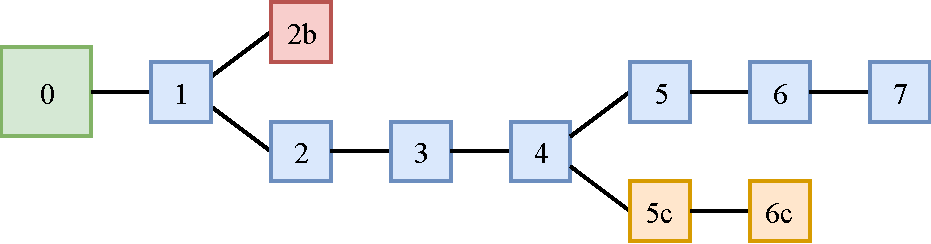
\includegraphics[scale=0.9]{figures/forks}
	\vspace*{0.25cm}
	\caption[Schematic representation of a blockchain with \num{3} branches.]{
		Schematic representation of a blockchain with \num{3} branches.
		The red block \texttt{2b} and the yellow blocks \texttt{5c} and \texttt{6c} are forks of the main chain that originate respectively at blocks \texttt{1} and \texttt{4}.
		Green blocks are on the longest chain, since block \texttt{7} is the one with the highest number of preceding blocks.
		The blue block represents represents the ``genesis''.
	}
	\label{fig:forks}
\end{figure}

Forks are probably the biggest problem in Bitcoin, since they allow an attacker to try to spend the money twice by creating two contrasting transactions that get stored in blocks published on different branches of the blockchain.
We will cover the ``double-spend'' attack in greater detail in \cref{chapter:attacks}.

\section{Mining \& Proof of Work}
\label{sec:mining}
The usage of modern cryptography in Bitcoin addresses and transactions guarantees that only the owner of some money can actually spend it (at least until the private key associated to the address is carefully protected).
Also, since all transactions are recorded and stored in the blockchain, the blockchain uses cryptographic hashes to detect tampering and it is replicated around many computer and devices around the world, it is very difficult or even impossible to remove old transactions from the past (i.e. revert payments).
However, there is so far no mechanism that prevents an attacker to create a big number of forks by simply forging new blocks.

\bigskip
Bitcoin uses \ac{PoW} \cite{pow_2002} to reduce the feasibility of such an attack.
It requires to solve a cryptographic puzzle and include its solution to create a valid block.
The difficulty of the puzzle is agreed by the network and depends on the total computational power available.
The puzzle consists in finding a nonce to include in the block such that the cryptographic hash of the serialized block is less than a target number, i.e. it starts with a certain number of zeros.
Thanks to the properties of cryptographic hash functions, the only way to solve the puzzle is a brute-force approach, which requires time and resources (in terms of both computation power and energy).
This mechanism prevents an attacker to forge too many blocks, since it would require too many resources and time.

\bigskip
People that manage to create a new block (miners) get a reward in bitcoins when the block is stored in the main chain;
also, they get the fees of all transactions stored in the block.
The address of the miner is stored in the header of the block, so the other nodes that run the Bitcoin protocol know who to acknowledge for both rewards.
It is important to notice that a miner is able to spend the reward obtained only if the corresponding block is stored in the main chain:
blocks in different branches of the blockchain are not recognized, since all correct nodes will only consider the longest (main) chain as valid.
Bitcoin rules try to encourage miners to behave correctly:
if a miner has a block stored in the blockchain, it is its interest to keep mining on the longest chain, in order to make more difficult or impossible for an attacker to create a branch which gets longer than the main chain, since this might ``cancel'' the rewards of the miner.

\bigskip
The process of mining in Bitcoin can be seen as a competition between miners.
As soon as a new block is created, it is published and appended to the longest branch in the blockchain.
Then, miners move the next block:
they choose the transactions to include from the one not yet processed, create the block by including the current timestamp, their address and the other information required and start to look for a nonce value that solves new the cryptographic puzzle.
When a miner finishes a block, all the others stop and start again from the longest branch:
it would make no sense to complete the current block\footnote{At least for honest miners (those that does not deviate from the Bitcoin protocol); malicious miners might have an advantage to choose a different strategy, as explained in \cref{chapter:attacks}}, since it would be in conflict with the current longest chain and would probably be ignored by the other nodes in the network.
The idea behind this strategy - which is the one implemented in official Bitcoin implementation originally created by Satoshi Nakamoto \cite{bitcoin_github} - is to waste as little computational power as possible:
when a block is attached to the longest chain, it would be a waste to complete another block that should be put in the same place as the first one.

\section{Mining Pools}
It is important to notice that the cryptographic puzzle used by Bitcoin is highly parallelizable, both on a single computer with a multi-core \ac{CPU} and as a distributed algorithms in a cluster of machines.
The only known way to solve the puzzle is a brute-force approach, which means trying all possible values for the nonce until a good nonce is found.
Also, since the nonce has a binary representation on a finite number of bits, it is trivial to partition the set of all possible values in ranges.
Each range can be assigned to a different core of the \ac{CPU} or distributed to a different machine in a cluster;
each core or machine reports the good nonces to some central coordinator, which it responsible to publish the block to the network and distribute new tasks to perform.

Because of the properties of cryptographic hash functions, the expected number of trials required to find a good nonce is $2^{b - 1}$, where $b$ is the number of bits in the binary representation of the nonce in a block header.
To verify if a nonce is good for a block, a miner only needs to put the nonce in the correct location in the block header and compute the hash function on the complete block.
The expected time to complete a block is thus proportional to the speed of the miner in computing an hash function.
This value is usually called ``Hash Rate'' in the Bitcoin vocabulary \cite{bitcoin_vocabulary}.

Miners are in competition with each other:
after a new block is published, honest miners start to work on the next block.
The probability of a miner to be the first one to complete a block is proportional to its hash rate.
Miners with small hash rates (e.g. those that use a general-purpose computer) are statistically very unlikely to ever find a block, and thus to earn a reward.
For this reason, miners to cooperate with each other in groups and create the so-called ``Mining Pools''.

\bigskip
A mining pool is a set of miners that share their computational power in the mining process.
Each pool has a coordinator that participates in the normal Bitcoin protocol:
it collects pending transactions, distribute blocks etc.
In addition, the coordinator creates ranges of nonces values and distributes them to the pool (as described above);
when a node finds a good nonce, it reports it to the coordinator, which completes and distributes the block to the rest of the Bitcoin network.
The same process is repeated for the next blocks.
The coordinator is also responsible for sharing the rewards among the nodes in the pool:
all blocks are created using the address of the coordinator, which collects all rewards, and periodically pays each node based on its contribution to the mining process.

Mining pools are a way to minimize the risk.
If the pool has a sufficient hash rate, it is likely to complete blocks before other miners and get the reward;
even small miners can contribute to a pool and get a small reward.

\bigskip
Mining pools use Stratum \cite{stratum}, a protocol introduces in \num{2012} to coordinate the mining process.
The protocol is based on plain HTTP \cite{stratum_manual}:
miners authenticate against the pools, but there is no verification of the pool's identity and the network traffic is in clear.
The pool coordinator and the miners communicate using JSON-RPC:
some commands are used to establish the initial connection between a miner and a pool (authenticate, reconnect, show message to the user, etc.), other commands are available to distribute mining tasks and collect the results.

\chapter{Protocol}
\label{chapter:protocol}
This chapter focuses on the low-level peer-to-peer protocol that runs Bitcoin.
Unfortunately, the Bitcoin protocol has never been documented properly:
the original paper \cite{bitcoin_2009} does not describe the details of the protocol and no official and complete description is available.
The single point of truth available is the open-source original Bitcoin client, \texttt{bitcoind} \cite{bitcoin_github}:
at the time of writing, around \num{95}\% of nodes in the network run some version of this client \cite{bitnodes}.
Unfortunately, the source code is quite hard to understand and contains almost no comment.
The content of this chapter is based primarily on academical papers \cite{eclipse_attack_2015, deanonymization_2014}, on some online references \cite{bitcoin_reference, bitcoin_guide} and only marginally on the source code itself.

\bigskip
Peers in the Bitcoin network are identified by their IP address.
Each node can initiate up \num{8} outgoing connections with other nodes, and accept up to \num{117} incoming connections, for a total of \num{125} \footnote{With the default settings (it is possible to configure custom values if necessary). Measures show that the majority of nodes have at most \num{8} outgoing connections and never reach the maximum number of incoming ones \cite{discovering_influential_nodes_2014}.}.
All connections use unencrypted TCP channels.
Nodes propagate and store only public IP addresses.
At the moment of writing, there are about \num{9000} reachable server, while the number of clients is estimated to be between \num{100000} and \num{200000}.
Nodes can also connect to the network via Tor \cite{bicoin_tor}.

\bigskip
We divide the description of the protocol in \num{2} parts: topology and core.
The former is responsible to create and maintain a peer-to-peer overlay network between Bitcoin nodes;
the latter uses the underlying overlay network to propagate blocks and transactions.

\section{Topology}
TODO

\subsection{Peers Discovery}
\label{sec:discovery}

\subsection{Bootstrap}
TODO

\subsection{Messages}
TODO

\paragraph{getAddr}
TODO

\paragraph{addr}
TODO

\section{Core}
TODO

\subsection{Messages}
TODO

\chapter{Attacks}
\label{chapter:attacks}
Various attacks has been performed against Bitcoin in the past.
Attacks can be performed at different levels with very different approaches and can have a wide range of effects on Bitcoin users.
This chapter starts from an overview of the most relevant ones.
At the end, it describes in details the Balance attack, whose analysis is the main object of the simulations.

\section{Double Spending}
\label{sec:double-spending}
Double-spending is the result of successfully spending some money more than once.
The attack is the oldest known one against Bitcoin and it is even partially discussed in the original Bitcoin paper \cite{bitcoin_2009}.
The attack has been analyzed many times in the literature \cite{double_spending_fast_payments, double_spending_two_for_one, double_spending_bitcoin_economics, double_spending_fast_analysis_2014} and has been reported to be quite easy to mount against fast payments \cite{double_spending_fast_payments}.
Real episodes of the attack has been reported multiple times in the past \cite{double_spending_ghash, double_spending_stackexchange}.
Double-spending breaks the most important guarantee that Bitcoin tries to give:
transactions are irreversible and bitcoins can be spent only once.

The attack works by creating \num{2} conflicting transactions (that spend all the bitcoins in the same address) and submitting them to different parties, for example \texttt{tx-1} to a merchant and \texttt{tx-2} to the Bitcoin network:
if the merchant accepts \texttt{tx-1} but the Bitcoin network receives \texttt{tx-2} before \texttt{tx-1}, it is likely that \texttt{tx-2} will be stored in the blockchain, while \texttt{tx-1} will be discarded, since not compatible with \texttt{tx-2}.
The attacker only pretends to spend some bitcoins to pay the merchant, but it actually does not spend anything:
it gets the purchase for free, while the merchant never receives the due bitcoins.
The double-spending attack can be performed directly in some cases, or it can be the result of more complex attacks.
There are many variants of double-spending, we analyze the most common ones here.

\subsection{Race Attack}
\label{sub:race-attack}
The race attack involves merchants that immediately accepts payments, without waiting for the unconfirmed transaction to be securely store in some block in the blockchain \cite{bitcoin_wiki_irreversible_transactions}.
The race attack has a high degree of success for an attacker \cite{double_spending_two_for_one}.
The attack is illustrated in \cref{fig:race-attack} and works as follows:
\begin{itemize}
	\item the attacker sends a transaction \texttt{tx-1} to the merchants;
	\item at the same time, the attacker sends a conflicting transaction \texttt{tx-2} to some miner; the conflicting transaction spend the bitcoins stored in the same address used in \texttt{tx-1} and sends them to new address in control of the attacker;
	\item the merchants sees the unconfirmed transaction and accepts the payment; this scenario is more likely for in-shop purchases, where, in many cases, the merchant can not wait for the transaction to be stored in the blockchain;
	\item \texttt{tx-2} is received before \texttt{tx-1} from the miners, so it is more likely to be stored in some block before \texttt{tx-1};
	\item \texttt{tx-2} is stored in a block, while \texttt{tx-1} is rejected since in conflict with \texttt{tx-1}.
	      % \item the attacker receives its bitcoins back, while the merchant does not get anything.
\end{itemize}

\begin{figure}[t]
	\centering
	\vspace*{0.25cm}
	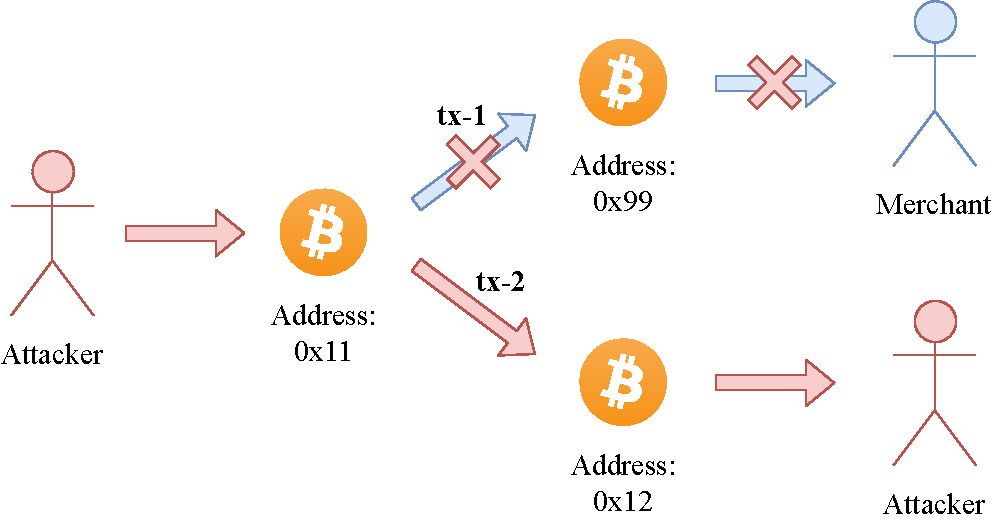
\includegraphics[scale=0.75]{figures/race_attack}
	\vspace*{0.25cm}
	\caption[Illustration of the race attack, a variant of double-spending]{
		Illustration of the race attack, a variant of double-spending.
		The attacker (in red) owns some bitcoins in the address \texttt{0x11}.
		It submits a transaction \texttt{tx-1} to move the money from its address \texttt{0x11} to the merchant's one \texttt{0x99} (in blue).
		At the same time, it submit to the Bitcoin network a conflicting transaction \texttt{tx-2} to move the the money from \texttt{0x11} to a new address \texttt{0x12} in its control.
		If the network includes \texttt{tx-2} in some block before \texttt{tx-1}, \texttt{tx-1} is rejected, and the money stay control of the attacker.
		The red arrows indicate the real flow of bitcoins, after that \texttt{tx-2} is stored in the blockchain and \texttt{tx-1} is rejected;
		the blue arrows with red crosses indicate what the correct flow of money would if the attack fails.
	}
	\label{fig:race-attack}
\end{figure}

A trivial defense for the merchant is to wait for the transaction \texttt{tx-1} to be stored in the blockchain:
if it is rejected because of any conflicts, the merchant can simply refuse the payment and do not sell the good.
Unfortunately, Bitcoin requires on average \SI{10}{minutes} to confirm a transaction, so this technique can not be always applied.
Bitcoin's developers recommendation is also to wait for \num{6} confirmations, i.e. to wait for the block that stored the transaction to be in the longest chain and to have \num{6} following blocks \cite{confirmation}.
Some blocks can be conflicting with each other (if they have the same parent):
only one of them can belong to the longest chain, while the others are said to be ``orphaned'' \cite{orphaned_block} and simply ignored, as illustrated in \cref{fig:orphaned-block}.
Thus, a transaction can be rejected even if it manages to get part of a block, if that block is orphaned.
Waiting for \num{6} confirmations gives a good tradeoff between the time to wait (on average \SI{1}{hour}) and statistical guarantee that the transaction is unlikely to be rejected later \cite{bitcoin_2009}.

\begin{figure}[ht]
	\centering
	\vspace*{0.25cm}
	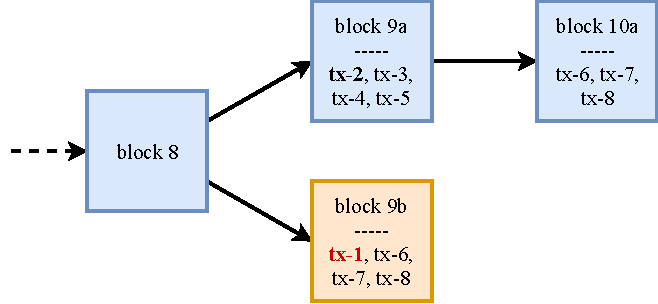
\includegraphics[scale=1.1]{figures/orphaned_block}
	\vspace*{0.25cm}
	\caption[Illustration of an orphaned block]{
		Illustration of an orphaned block.
		Blocks \texttt{9a} and \texttt{9b} have the same parent.
		Since \texttt{9a} has a child \texttt{10a}, it is on the longest chain.
		Transactions \texttt{tx-6}, \texttt{tx-7} and \texttt{tx-8} from the orphaned block \texttt{9b} are stored in \texttt{10a};
		\texttt{tx-1} (in red) is in conflict with \texttt{tx-2} and is thus rejected.
	}
	\label{fig:orphaned-block}
\end{figure}

\subsection{Finney Attack}
The Finney attack is another variant of double-spending targeting merchants that accepts unconfirmed payments.
It can be performed by an attacker that is able to mine some blocks.
The attack works as follows:
\begin{itemize}
	\item the attacker controls addresses \texttt{addr-a} and \texttt{addr-b};
	\item the attacker mines a new block on the longest chain; the block includes a transactions \texttt{tx-2} that moves all bitcoins from address \texttt{addr-a} to \texttt{addr-b};
	\item before broadcasting the block to the Bitcoin network, the attacker sends a transaction \texttt{tx-1} to a merchant, spending again the bitcoins in \texttt{addr-a};
	\item as soon as the merchants accepts the payment, the attacker broadcasts its block to the network;
	\item \texttt{tx-2} is stored in the blockchain before \texttt{tx-1}, so \texttt{tx-1} is rejected because in conflict with \texttt{tx-2};
	\item the attacker receives its bitcoins back, while the merchant does not get anything.
\end{itemize}
Similarly to the Race attack, the Finney attack relies on conflicting transactions and the significant time required to confirm a transaction with a high confidence in Bitcoin.
The defense for the merchant is the same discussed in \cref{sub:race-attack}.

\section{Majority Attack}
\label{sec:majority-attack}
The majority attack, also known as \num{51}\% attack, refers to a situation in which one miner (or one group of miners) control more that \num{50}\% of the entire network's mining hash rate \cite{majority_investopedia, majority_bitcoin_wiki}.
An attacker with such a computational power can generate blocks faster than the rest of the network:
it can potentially take control of the entire blockchain and each block in the longest chain.
The attacker strategy is to mine its private chain, ignoring the current longest chain and each block honest miner published.
This strategy gives statically guarantees to eventually generate the longest chain, no matter the advantage of honest miners (in terms of the difference in the number of blocks on the current longest chain and the number of blocks in the attacker's chain).
Such an attacker could, potentially, start its own chain from the genesis block and revert the entire history of Bitcoin, as illustrated in \cref{fig:majority-attack}.

There is no defense against this attack:
Bitcoin's security relies on an honest majority of nodes that collectively control more computational power than any attacker (or group of attackers) \cite{bitcoin_2009}.
To be more precise, the system is not vulnerable to the majority attack as long as no single coalition of miners controlling more than \num{50}\% of the total hash rate \cite{bitcoin_wiki_irreversible_transactions}.

\begin{figure}[t!]
	\begin{subfigure}{\textwidth}
		\centering
		\vspace*{0.25cm}
		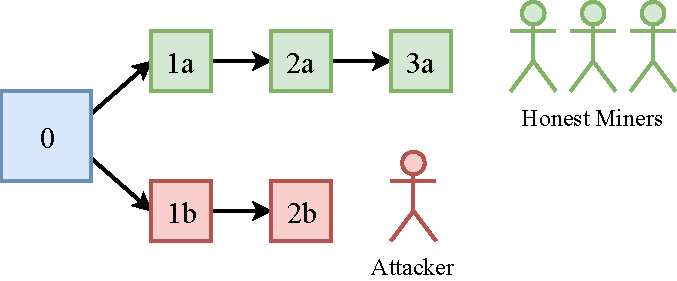
\includegraphics[scale=0.9]{figures/majority_attack_1}
		\vspace*{0.25cm}
		\caption{
			The attacker starts to mine block (in red) from the genesis (number \texttt{0}, in blue) instead of following the longest chain (in green).
			Honest miners keep following the green chain that finishes with block \texttt{3a}.
		}
		\vspace*{0.75cm}
	\end{subfigure}
	\begin{subfigure}{\textwidth}
		\centering
		\vspace*{0.25cm}
		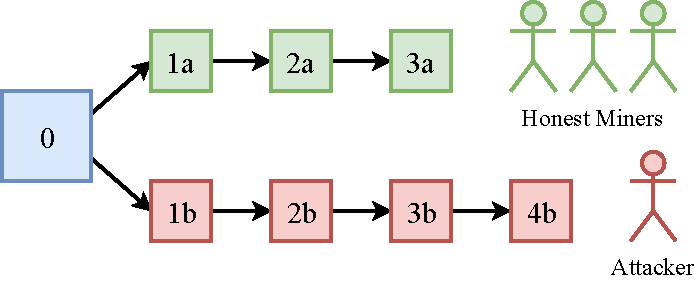
\includegraphics[scale=0.9]{figures/majority_attack_2}
		\vspace*{0.25cm}
		\caption{
			Eventually, the attacker's chain gets longer than the previous longest chain.
			The attacker broadcasts all blocks in his chain to the Bitcoin network.
		}
		\vspace*{0.75cm}
	\end{subfigure}
	\begin{subfigure}{\textwidth}
		\centering
		\vspace*{0.25cm}
		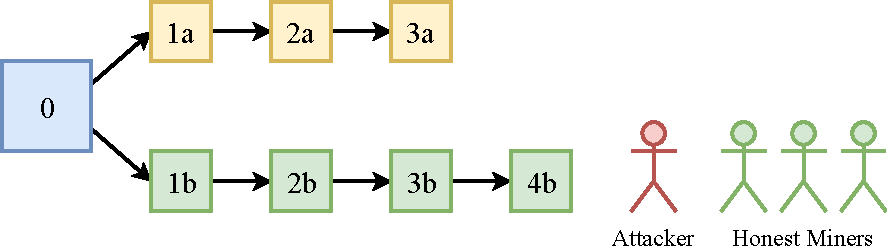
\includegraphics[scale=0.9]{figures/majority_attack_3}
		\vspace*{0.25cm}
		\caption{
			Honest miners start following the attacker's chain (now in green), since it is not longer than the chain terminating with block \texttt{3a}.
			The oldest chain (now in yellow) is orphaned: all transactions stored in blocks \texttt{1a}, \texttt{2a} and \texttt{3a} are not valid anymore.
			Potentially, the attacker may include transactions conflict with the canceled once in any of the new blocks \texttt{1b}, \texttt{2b}, \texttt{3b} and \texttt{4b}, effectively double-spending some or all of its bitcoins.
		}
		\vspace*{0.25cm}
	\end{subfigure}
	\caption[Illustration of the different phases of a majority attack]{
		Illustration of the different phases of a majority attack, where an attacker takes control of the entire blockchain, starting from the genesis block.
		The attacker is able to revert the history of all transactions stored in the blockchain.
	}
	\label{fig:majority-attack}
\end{figure}

The majority attack allows an attacker to perform the following actions \cite{weaknesses_bitcoin_wiki}:
\begin{itemize}
	\item rewrite the history of the blockchain;
	\item prevent some or all transactions from becoming part of the longest chain;
	\item prevent some or all other miners from attaching new blocks to the longest chain (and thus getting any reward);
	\item reverse transactions it has made in the past, effectively double-spending its bitcoins;
	\item gain the revenue of all new blocks.
\end{itemize}

A majority attack can completely destroy the working of Bitcoin and violate some of its main guarantees (e.g. spending the same bitcoins only once).
Such an attack is thought to be very unlikely \cite{ghash_never_51_attack_cex, ghash_never_51_attack_coindesk}, because of its huge cost in terms of computing power and the risk for an attacker not to gain anything from it:
even if it is theoretically possible to revert all blocks following the genesis, it is incredible expensive.
The attack would immediately destroy the credibility of Bitcoin and lead to the following \num{2} possible effects:
\begin{enumerate}
	\item the value of bitcoins drops completely, and the attacker does not earn any real reward;
	\item the rules of the Bitcoin software are changed by the community to revert the attack \cite{weaknesses_bitcoin_wiki}.
\end{enumerate}

% TODO: this makes formatting better...
\pagebreak

In January 2014, the mining pool \texttt{GHash.IO} reached \num{42}\% of the total Bitcoin hash rate \cite{ghash_fears_51_attack, security_survey_2017}, and later in July 2014 it exceeded the threshold of \num{51}\% \cite{wikipedia_ghash, majority_investopedia, bitcoin_wiki_irreversible_transactions}.
Even though there is no evidence of a majority attack to ever been mounted against Bitcoin, the episode was quite controversial in 2014:
a number of miners voluntarily dropped out of the pool and \texttt{GHash.IO} implemented a mechanism to prevent the situation to ever happen again in the future \cite{ghash_51_percent_extremetech, ghash_commits_to_40_percent_coindesk, ghash_commits_to_40_percent_arstechnica}.

\section{Selfish Mining}
\label{sec:selfish}
Selfish Mining \cite{selfish_mining_acm} is a strategy where a group of miners strategically chooses when to submit the new blocks to the public chain, rather than submitting them immediately upon discovery.
The selfish miners keep the discovered blocks private, intentionally forking the blockchain and mining on their own private branch.
The honest nodes do not know about the blocks discovered by the selfish miners, so they continue to mine on the public chain.
If the public longest chain approaches the selfish miners' private branch length, they reveal some blocks to surpass the public chain again.
The selfish miners causes the honest miners to waste a lot of computational power on obsolete chains, since the longest one is not yet public.
The idea is illustrated in \cref{fig:selfish-mining}.

\begin{figure}[h!]
	\begin{subfigure}{\textwidth}
		\centering
		\vspace*{0.25cm}
		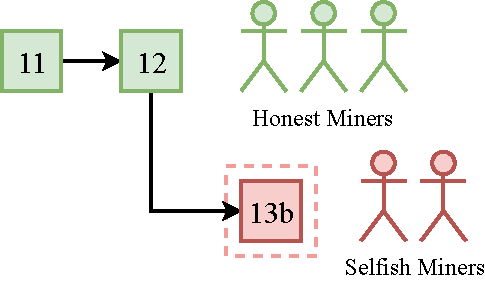
\includegraphics[scale=0.9]{figures/selfish_1}
		\vspace*{0.25cm}
		\caption{
			The selfish miners secretly mine block \texttt{13b} from the current public longest chain (in green).
			The honest miners do not know about block \texttt{13b}, so they keep working from block \texttt{12}.
		}
		\vspace*{0.75cm}
	\end{subfigure}
	\begin{subfigure}{\textwidth}
		\centering
		\vspace*{0.25cm}
		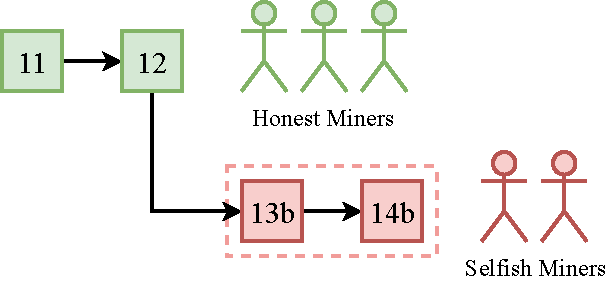
\includegraphics[scale=0.9]{figures/selfish_2}
		\vspace*{0.25cm}
		\caption{The selfish miners manage to secretly mine another block \texttt{14b} and keep it secret (secret blocks are indicated by the red dashed box).}
		\vspace*{0.75cm}
	\end{subfigure}
	\begin{subfigure}{\textwidth}
		\centering
		\vspace*{0.25cm}
		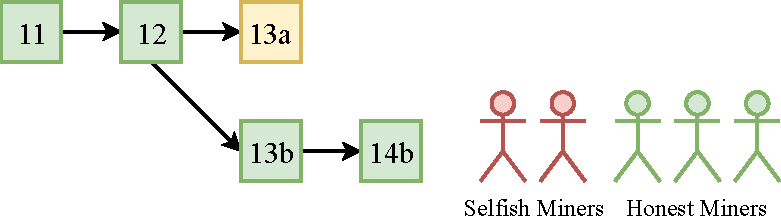
\includegraphics[scale=0.9]{figures/selfish_3}
		\vspace*{0.25cm}
		\caption{
			Honest miners manage to mine block \texttt{13a} and publish it.
			Selfish miners reveal the secret chain, which is longer than the public longest chain.
			Honest miners discard block \texttt{13a} (in yellow) and start to follow the new longest chain (block \texttt{14b}).
			The computational power used to mine block \texttt{13a} gets wasted and the honest miners do not get any revenue.
		}
		\vspace*{0.25cm}
	\end{subfigure}
	\caption[Illustration of the Selfish Mining strategy]{Illustration of the Selfish Mining strategy.}
	\label{fig:selfish-mining}
\end{figure}

Selfish Mining has been proposed in 2013 by Ittay Eyal and Emin G\"un Sirer \cite{selfish_mining}.
In their paper, they show that both the selfish and the honest miners waste some resources, but the honest miners waste proportionally more:
overall, the rewards share for the selfish miners is higher than the proportion of computational power they own.
In practice, this gives the selfish miners an advantage over the others and encourages rational miners to join the group of selfish miners.
According to the paper, relatively small group of miners can adopt the selfish strategy and attract many other miners, with the risk of gaining the majority of the mining power (see \cref{sec:majority-attack}).

\medskip
Some work has been done in academics to investigate alternative mining strategy \cite{other_mining_strategies_2014, block_hiding_strategies_2014}.

Nayak Kartik et at. have proposed Stubborn Mining \cite{stubborn_mining_2016}, a strategy heavily inspired by Selfish Mining, but that accepts some more risk (e.g. keep mining on chains shorter than the longest one) in return to a higher expected revenue.
They claim that stubborn mining strategies can beat Selfish Mining by up to \num{25}\%.

Ayelet Sapirshtein, Yonatan Sompolinsky and Aviv Zohar have investigated the space of possible selfish mining strategies, looking for the optimal strategy for selfish miners \cite{optimal_selfish_mining_2016}.
They also show that selfish mining strategies can be combined with double-spending attempts to make them even more profitable for selfish miners.


\section{Eclipse Attack}
\label{sec:eclipse}
The general idea of the Eclipse Attack \cite{eclipse_overlay_2006} is to force a victim to connect only nodes under the control of the attacker:
if the attacker succeeds in doing that, it is able to control all the network traffic to and from the victim.
In the specific case of Bitcoin, the attacker can mount many different attacks against the victim, for example a double-spending against a merchant.

\begin{figure}[h!]
	\begin{subfigure}{.45\textwidth}
		\vspace*{0.25cm}
		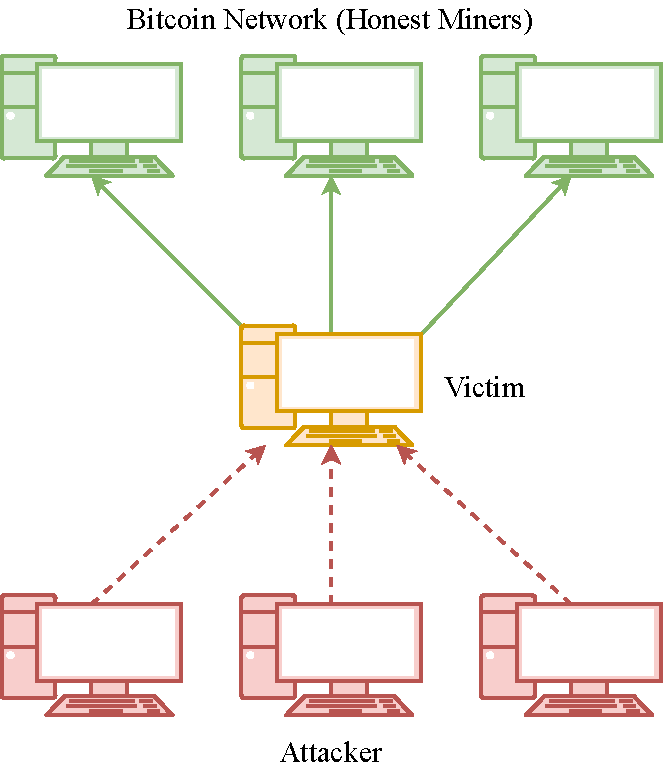
\includegraphics[width=\columnwidth]{figures/eclipse_1}
		\vspace*{0.1cm}
		\caption{
			At the beginning, the victim is connected to some honest miners in the Bitcoin network.
			The attacker opens new connections against the victim from many different malicious nodes under its control.
			If the attack succeeds, the victim will eventually forget the addresses of honest nodes and fill its tables with addresses of malicious nodes.
		}
	\end{subfigure}
	\hfill
	\begin{subfigure}{.45\textwidth}
		\vspace*{0.25cm}
		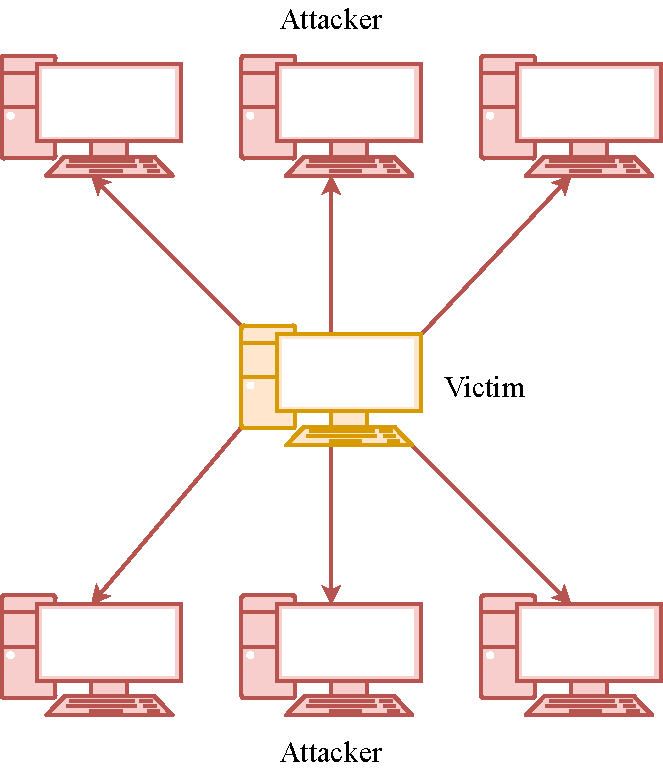
\includegraphics[width=\columnwidth]{figures/eclipse_2}
		\vspace*{0.1cm}
		\caption{
			When the victim reboots, it connects to known nodes.
			Since its tables are full of addresses of hosts under the control of the attacker, the victim will connect only to malicious nodes.
			The attacker can now decide which messages to forward to the victim and which not to:
			the attacker can effectively eclipse the victim from the peer-to-peer network.
		}
	\end{subfigure}
	\caption[Illustration of an Eclipse Attack]{Illustration of an Eclipse Attack.}
	\label{fig:eclipse}
\end{figure}

\medskip
Each Bitcoin node maintains \num{2} tables of addresses \cite{eclipse_attack_2015}:
the \texttt{tried} table contains addresses of peers that were successful connected with the current node at least one in the past;
the \texttt{new} table contains addresses discovered through any of the peers-discovery strategies used by Bitcoin (see \cref{sub:discovery}) to whom the node has not yet initiated a successful connection.

A Bitcoin running the original client \cite{bitcoin_github} with the default settings can have up to \num{8} outgoing and up to \num{117} unsolicited incoming connections, for a total of \num{125} \cite{deanonymisation_2014, eclipse_attack_2015} (see \cref{chapter:protocol} for the details).
Connections are long-lived, i.e. they are interrupted only if either one of the \num{2} nodes goes down or in case of networking problems.
Each Bitcoin node always tries to have exactly \num{8} outgoing connections, in order to maintain a solid network topology.
If the number of outgoing connections gets less than \num{8}, the node randomly chooses a new IP address from the \texttt{new} table and tries to connect to the corresponding node:
if the connection is not successful, the node tries with the next address.

\medskip
An Eclipse Attack against Bitcoin \cite{eclipse_attack_2015} is illustrated in \cref{fig:eclipse} and works as follows:
\begin{itemize}
	\item the attacker rapidly and repeatedly opens new unsolicited connections to the victim from a set of malicious nodes under its control; when a new connection is establishes, the attacker also sends unsolicited \texttt{Addr} messages containing a list of up to \num{1000} ``trash'' addresses (IPs of host that do not run Bitcoin or addresses under the control of the attacker);
	\item if the attack succeeds, the victim will eventually replace all addresses stored in both the \texttt{tried} and the \texttt{new} tables with the IP addresses of the malicious nodes;
	\item the attacker forces the victim to restart \cite{cve_bloom_filter_2013, bitcoin_common_vulnerabilities} or simply waits for it to restart naturally, for example after a software update or after some failure;
	\item when the victim restarts, it will connect to \num{8} malicious nodes randomly chooses from the \texttt{tried} and the \texttt{new} tables;
	\item the attacker effectively isolates the victim from the honest nodes in the network and can control which messages, block and transactions to relay, delay or drop.
\end{itemize}

The attacker can mount many different attacks against eclipsed nodes.
If the victim is a miner (or a mining pool), the attacker can adopts strategies similar to the Selfish Mining to waste the computing power of the eclipsed nodes:
the attacker can drop \texttt{Block} messages containing blocks discovered by the victim and forward blocks from the network that conflict with the ones found by the victim.
If the victim is a merchant, the attacker can easily mount double-spending attacks.
It can send a transaction \texttt{tx-1} to the merchant, and a conflicting one \texttt{tx-2} to the Bitcoin network:
since the attacker controls all of merchant's connections, the merchant might not be able to broadcast \texttt{tx-1} to the network and the attacker might be able to double-spend its bitcoins with \texttt{tx-2}.


\section{BGP Hijacking}
\ac{BGP} is a standardized network protocol used to exchange routing information between \ac{AS} \cite{autonomous_systems_wikipedia} of different \ac{ISP} and organizations on the Internet \cite{rfc4271, bgp_wikipedia}.
The primary function of \ac{BGP} is to exchanges information about network reachability with other \ac{BGP} systems.
The information collected and distributed by the protocol are used to construct a graph of connectivity between different \ac{AS}, which can be used to make optimal routing decisions among the networks of different parties.
\ac{BGP} routing also depends on policies and rules configured by network administrators.

\medskip
While not directly related to Bitcoin, \ac{BGP} is fundamental for the working of Internet, and thus for each distributed systems build on top of that.
Under some conditions, attacks against \ac{BGP} can affect Bitcoin and mine some of the guarantees given by the protocol.
Researchers at Dell SecureWorks Counter Threat Unit discovered an attacker that repeatedly hijacked traffic destined to networks belonging to Amazon, Digital Ocean, OVH, and other large hosting companies between February and May 2014 \cite{bgp_hijacking_secureworks}:
they registered \num{51} compromised networks from \num{19} different \ac{ISP}.
Attacks with a similar scale were also reported between October 2015 and April 2016 \cite{hijacking_bitcoin_2017, bgpstream}.

% TODO: this makes formatting better...
\pagebreak

\begin{figure}[h!]
	\begin{subfigure}{\textwidth}
		\centering
		\vspace*{0.25cm}
		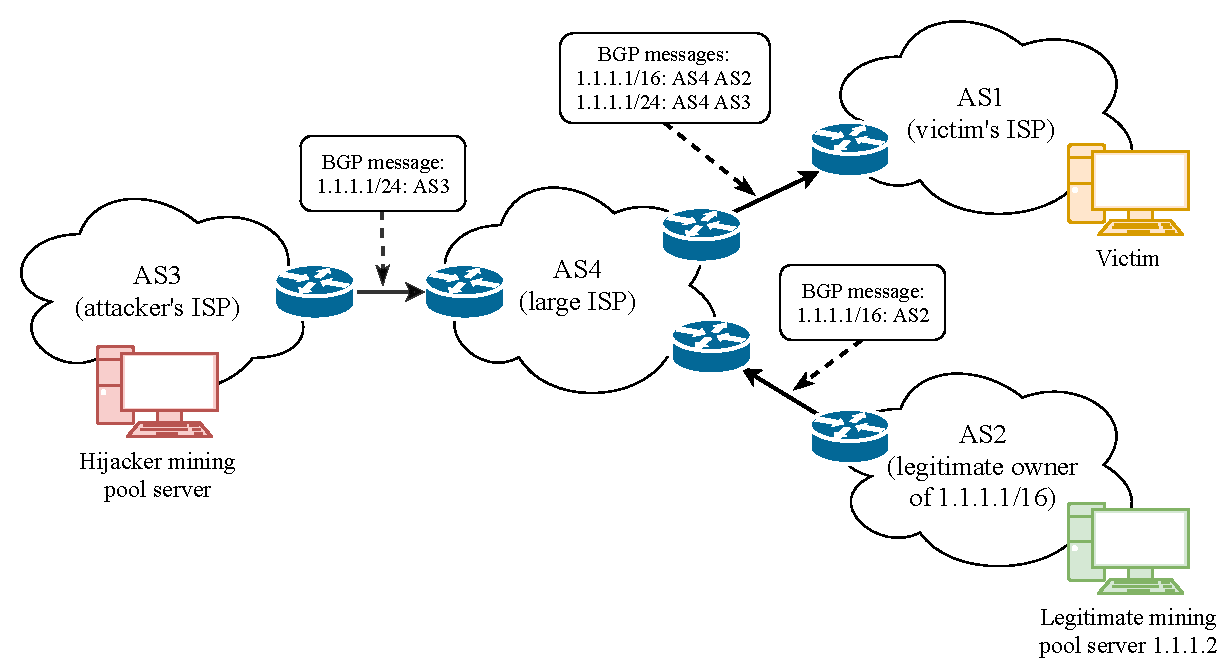
\includegraphics[width=\columnwidth]{figures/bgp_1}
		\vspace*{0.25cm}
		\caption{
			Broadcast of the malicious route.
			The legitimate miner (in green) has IP address \texttt{1.1.1.2} on the network \texttt{1.1.1.1/16} of \texttt{AS2}.
			\texttt{AS2} broadcasts its networks to the neighboring \ac{AS}.
			The attacker (in red) tries to hijack the victim's connection:
			since \texttt{AS4} is paired with \texttt{AS3}, the BGP message from the attacker is accepted.
			The malicious route is more specific than the legitimate one, so it is overridden in the \texttt{AS4} routing tables.
		}
		\vspace*{0.25cm}
	\end{subfigure}
	\begin{subfigure}{\textwidth}
		\centering
		\vspace*{0.25cm}
		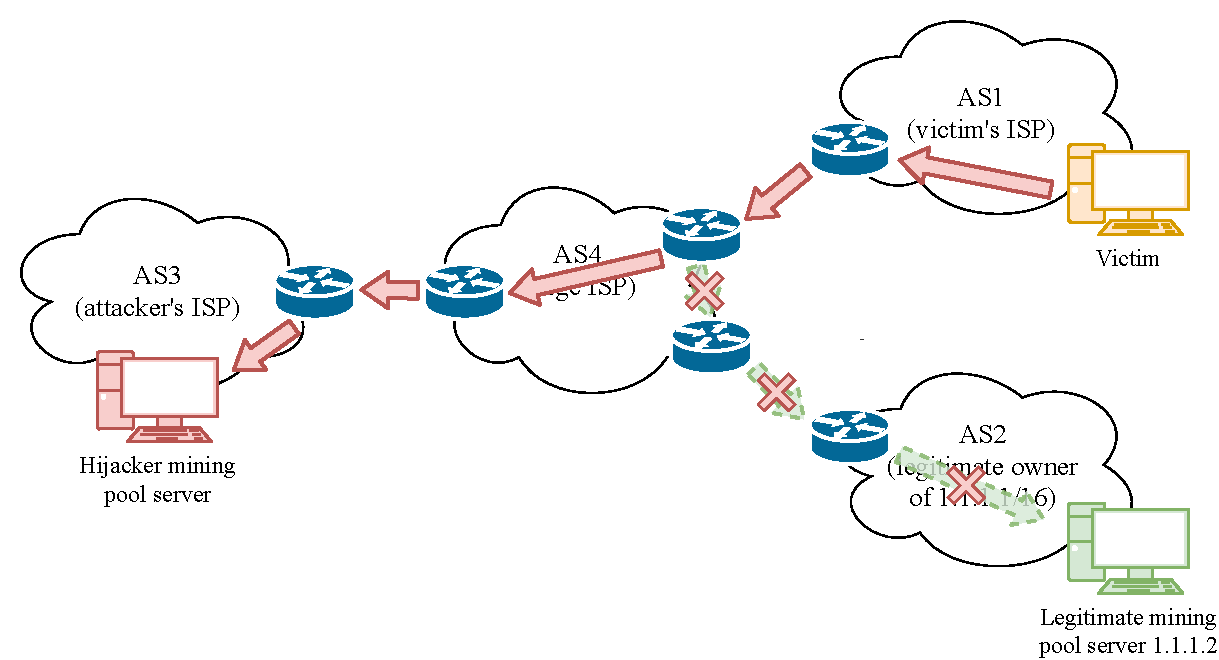
\includegraphics[width=\columnwidth]{figures/bgp_2}
		\vspace*{0.25cm}
		\caption{
			The victim tries to connect to the legitimate mining pool server at IP \texttt{1.1.1.1}.
			The IP packets are correctly routed to \texttt{AS4}, but then \texttt{AS4} sends them to \texttt{AS3} instead of \texttt{AS2}:
			the victim connects to the attacker instead.
			The routing is indicated with red arrows;
			green arrows with red crosses indicate what the correct routing would be.
		}
		\vspace*{0.25cm}
	\end{subfigure}
	\caption[Illustration of a BPG Hijacking attack against a Bitcoin miner]{Illustration of a BPG Hijacking attack against a Bitcoin miner.}
	\label{fig:bpg-hijacking}
\end{figure}

A \ac{BGP} attack requires a malicious \ac{AS} and some manual configuration.
A network administrator of the malicious \ac{AS} must configure \ac{BGP} to announce wrong ranges of IP addresses:
the other \ac{AS} will learn wrong routes and override the correct routing rules.
If the attack is successful, some Internet traffic destined to the hijacked networks goes through the malicious \ac{AS} and can thus be intercepted, analyzed and manipulated by the attacker in any ways.
Since all the Bitcoin traffic is in clear and there in no authentication between different peers, Bitcoin is vulnerable to hijacking \cite{hijacking_bitcoin_2017}.
Similarly, traffic of the Stratum protocol used in by mining pools is vulnerable to routing attacks.

\medskip
\cref{fig:bpg-hijacking} shows an example of \ac{BGP} hijacking used against a Bitcoin miner running the Stratum protocol.
The attack works as follows:
\begin{itemize}
	\item the miner continuously connects to a legitimate pool, asking for tasks to perform;
	\item the attacker publishes new \ac{BGP} routes to intercept the victim's Stratum network traffic;
	\item when the miner attempts to connect to a legitimate pool, some \ac{BGP} route directs the traffic to a pool controlled by the attacker;
	\item the malicious pool issues a \texttt{client.reconnect} \cite{stratum_manual} command to instruct the miner to connect to a new pool maintained by the attacker;
	\item the victim connects to the second malicious pool;
	\item the attacker ceases the attack, since \ac{BGP} hijacking is not needed anymore at this stage;
	\item the miner performs the assigned tasks correctly, but does not get any revenue from the malicious pool, effectively wasting its computing power for free.
\end{itemize}

\medskip
In the paper ``Hijacking Bitcoin: Routing Attacks on Cryptocurrencies'', Maria Apostolaki et at. show that large scale networks attack against Bitcoin are possible and have been already done in the past.
They claim that anyone with access to a BGP-enabled network and able to hijack less than \num{900} prefixes (about \num{0.15}\% of the total) can perform attacks commonly believed to be hard, such as isolating \num{50}\% of the mining power.
Attackers controlling some networks can potentially:
\begin{itemize}
	\item force miners to connect to a malicious pool which exploits their mining power for free;
	\item isolate part of the network by delaying or dropping messages to or from the victims (see the Eclipse Attack described in \cref{sec:eclipse});
	\item perform double-spend attacks against merchants;
	\item take control of a significant amount of computing power and attempt various kind of mining attacks (see \cref{sec:selfish}).
\end{itemize}


\section{Balance Attack}
\label{sec:balance}
The Balance attack is a new attack proposed by Christopher Natoli and Vicent Gramoli first in \num{2016} in the technical report \cite{balance_attack_report_2016} and later in \num{2017} in their paper ``The Balance Attack or Why Forkable Blockchains Are Ill-Suited for Consortium'' \cite{balance_attack_2017}.
The attack targets \textit{forkable} blockchains, i.e. a blockchain that allow multiple branches at the same time.
The most famous examples of systems using a forkable blockchains are Bitcoin \cite{bitcoin_2009} and Ethereum \cite{ethereum_2014}.

\medskip
Forkable blockchains implement some strategy to solve conflicts:
for example, Bitcoin always follows the longest chain if multiple branches exists.
The rule guarantees that the system will eventually agree on the same longest chain, and thus on the same set of transactions stored in the blockchain.
Unfortunately, blocks in branches different from the longest chain are wasted, since their content is not recognized by the network.
Wasted blocks are probably the biggest problem of forkable blockchains:
they waste computational power of the network and facilitate double-spending attacks \cite{double_spending_fast_analysis_2014}.

Except for attacks, network delays are the main cause of forks in the blockchain \cite{information_propagation_2013}.
Honest miners immediately stop the mining process if they receive a new valid block that attaches to the longest chain and they start to mine the following block;
the delay between a block discovery and its broadcast may allow other miners to complete and publish a conflicting block, effectively creating a fork in the blockchain.
In practice, an attacker can increase the amount of wasted blocks in the system and slow down the growth of the longest chain by simply delaying the propagation of new blocks \cite{balance_attack_2017}.

\medskip
The Balance attack takes advantage of this idea.
The attacker partitions the Bitcoin nodes by disrupting communications between different subgroups:
the messages containing new blocks are delayed or possibly dropped completely.
The paper suggests to select groups of similar computing power to maximize the probability of success of the attack.
\cref{fig:balance} shows an example of Balance attack, where the attacker controls one router and is able to filter and manipulate traffic for the nodes connected to Internet through that router.
Multiple results recently demonstrated how simply a motivated attacker can perform networking attacks on the Internet and thus delaying messages in blockchain networks \cite{bgp_hijacking_secureworks, eclipse_attack_2015, hijacking_bitcoin_2017}.

\begin{figure}[h]
	\centering
	\vspace*{0.25cm}
	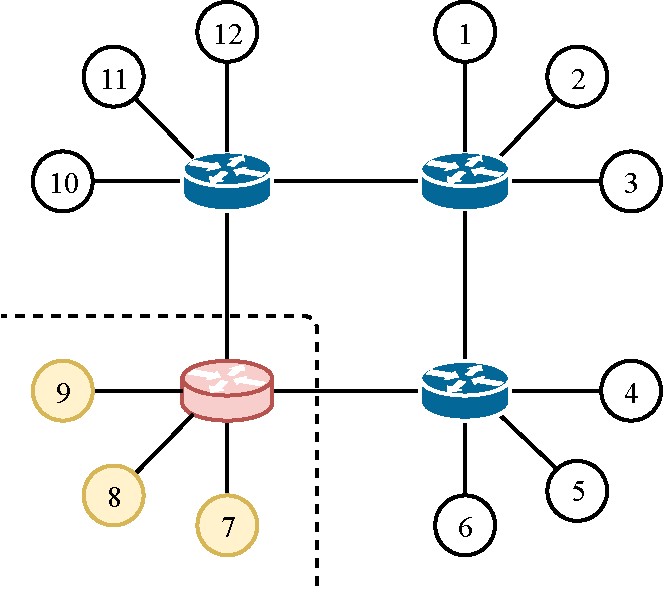
\includegraphics[scale=0.8]{figures/balance}
	\vspace*{0.25cm}
	\caption[Illustration of a network partitioning caused by a Balance Attack]{
		Illustration of a network partitioning caused by a Balance Attack.
		The attacker controls the bottom-left router (in red) and delays all communications between pair of nodes $(a, b)$ where $a \in \{7,8,9\}$ and $b \not \in \{7, 8, 9\}$:
		nodes inside the same partition can communicate with each other without any delay.
	}
	\label{fig:balance}
\end{figure}

In details, the attack works as follows:
\begin{itemize}
	\item the attacker identifies subgroups of miners with a similar mining power; different works in the literature \cite{deanonymization_2014, discovering_influential_nodes_2014} describe techniques to learn the network topology and identify influential nodes;
	\item the attacker identifies the routes of Bitcoin messages between different subgroups over Internet; let us assume the miner finds a partitions of nodes into \num{2} groups \texttt{G1} and \texttt{G2};
	\item the attacker runs some networking attack (man-in-the-middle, BGP hijacking \cite{bgp_hijacking_secureworks}) to take control of the communications links between groups and delays the Bitcoin traffic;
	\item because of the delay, transactions and blocks are not immediately propagated to the entire network, so \texttt{G1} and \texttt{G2} are very likely to have different views of the blockchain and to mine conflicting blocks;
	\item the attacker takes advantage of these inconsistencies and performs double-spending attacks.
\end{itemize}

The authors implemented and tested the attack against a private Ethereum test network with characteristics similar to \texttt{R3}, a consortium of more than \num{70} word-wide financial institutions.
The testnet consisted of \num{18} machines running Ethereum and mining blocks (the mining process in Ethereum is based on \ac{PoW} and is similar to the one of Bitcoin, at least for the matter of the Balance attack).
The authors report that a single machine needs to delay messages for \num{20} minutes to double spend, while an attacker controlling a third of the mining power only needs a delay of \num{4} minutes to achieve \num{94}\% of attack success rate.

\chapter{Simulator}
\label{chapter:simulator}

Testing and evaluating a peer-to-peer protocol with thousands of nodes in a real environment is very difficult, expensive and time consuming, especially if the goal is to evaluate the effects of large-scale network attacks.
For this reason, we decided to implement a simulator to measure the performances of the Bitcoin protocol under the different situations, at rest and under attack.
This allowed us to simulate up to \num{8000} Bitcoin nodes on a single general-purpose computer in a short time and evaluate the behavior of the protocol under different attack scenarios.

\medskip
This chapter describes the implementation of the simulator.
It covers the main concepts of discrete event simulation, the basics of PeerSim, the design of the simulator, the simplifications with respect to the complete Bitcoin protocol, and the metrics used to measure and evaluate the overall performances.


\section{Simulation}
According to Robert E. Shannon, \textit{simulation} is ``the process of designing a model of a real system and conducting experiments with this model for the purpose of understanding the behavior of the system and / or evaluating various strategies for the operation of the system'' \cite{simulation_shannon_1998}.
By \textit{model}, he means an abstract representation of an entity of group of objects, and by \textit{system} a collection of elements that interact with each other to accomplish some objective.
According to Shannon, simulation has a number of advantages \cite{simulation_shannon_1998}:
\begin{itemize}
	\item it is often easier to understand than analytical or mathematical models;
	\item it is usually more credible than models, since it requires less simplifying assumptions and represents the system more accurately;
	\item it allows to test new designs, systems or protocols before implementing them;
	\item it allows to verify hypothesis by measuring their effects on the systems;
	\item it helps to understand better how the modeled system works and which variables are the most important with respect to the performances;
	\item it allows to changes the initial situation and test the system in different settings.
\end{itemize}

\medskip
Simulation is used in many contexts, for example safety engineering, economics, physics and even video games \cite{wikipedia_simulation}.
There are many different approaches to simulations, each one adapted to a specific purpose.
We focus on discrete event simulation, used by our simulator.


\section{Discrete event simulation}
A discrete event simulation models the system behavior as a discrete sequence of events in time.
An event can represent anything, for example the arrival of a message to a node in the system or a network timeout.
Each event occurs at a particular instant of time and can cause changes in the state of the system.
No event occurs between \num{2} consecutive events, so the simulation can simply jump from one event to the next.
The results of the simulation can be evaluated with measurements:
the metrics can be computed either online during the simulation run, or computed offline from the simulation logs.

\medskip
\begin{algorithm}[h]
	\setstretch{1.15}
	\DontPrintSemicolon

	\SetKw{New}{new}
	\SetKwData{State}{state}
	\SetKwData{Events}{events}
	\SetKwData{Queue}{queue}
	\SetKwData{Event}{event}
	\SetKwData{NewState}{newState}
	\SetKwData{NewEvents}{newEvents}
	\SetKwFunction{InitializeState}{initializeState}
	\SetKwFunction{InitializeEvents}{initializeEvents}
	\SetKwFunction{PriorityQueue}{PriorityQueue}
	\SetKwFunction{IsEmpty}{isEmpty}
	\SetKwFunction{DeleteMin}{deleteMin}
	\SetKwFunction{InsertAll}{insertAll}
	\SetKwFunction{ProcessEvent}{processEvent}
	\SetKwFunction{ExitConditionReached}{exitConditionReached}

	\BlankLine
	\CommentSty{// initialization} \;
	\State $\leftarrow$ \InitializeState{} \;
	\Events $\leftarrow$ \InitializeEvents{} \;
	\Queue $\leftarrow$ \New \PriorityQueue{\Events} \;

	\BlankLine
	\BlankLine
	\CommentSty{// simulation loop} \;
	\While{$\neg$ \Queue.\IsEmpty{} or \ExitConditionReached{\State}}{

		\BlankLine
		\CommentSty{// process the next event} \;
		\Event $\leftarrow$ \Queue.\DeleteMin{} \;
		\NewState, \NewEvents $\leftarrow$ \ProcessEvent{\Event} \;

		\BlankLine
		\BlankLine
		\CommentSty{// update the system status} \;
		\State $\leftarrow$ \NewState \;
		\Queue.\InsertAll{\NewEvents} \;

		\BlankLine
	}
	\BlankLine

	\caption{Discrete Event Simulator}
	\label{alg:des}
\end{algorithm}
\smallskip

\cref{alg:des} illustrates the working of a discrete event simulation engine.
The simulation has some starting state that represents the initial condition of the system.
All events are stored in a priority queue sorted by event time.
The queue is initialized with some events.
Events in the queue are processed one at a time:
the first event is removed from the queue and processed by the simulator.
An event can cause other events to occur in the future and change the current state if the system.
Discrete event simulators take advantage of pseudorandom number generators to emulate random variables of the system \cite{wikipedia_des}:
whenever an event is influenced by some random factor external to the system (e.g. latency of a TCP connection over the Internet), the simulator extracts a random variable from some distribution using the random number generators.
The simulation stops when a certain condition is reached (for example, a target simulation time is reached), or when the queue of events is empty.


\section{PeerSim}
PeerSim \cite{peersim_2009} is an open source peer-to-peer systems simulator engine developed at the University of Bologna and the University of Trento.
It is written in Java and aim is to help the research and evaluation of large peer-to-peer.
It has been developed with high scalability in mind, in order to support simulations with up to \num{1} million nodes.
It is released under the GPL open source license and is available for download on SourceForce \cite{peersim_site}.

\smallskip
PeerSim is composed of two simulation engines, a simplified (cycle-based) one and an event-driven one.
The cycle-based engine uses some simplifying assumptions to achieve better performances and scalability, such as ignoring the details of the transport layer in the communication protocol stack;
it has been tested up to \num{1} million nodes \cite{peersim_intro_2018}.
The event-based engine is less efficient but more realistic and allows to easily simulate the entire network stack;
it has been used for simulation of up to \num{250000} nodes \cite{peersim_intro_2018}.
Both engines support many simple and extendable components, which are plugged together through a flexible configuration mechanism.
Since our simulator is event driven, this chapter focuses on the event-based engine only.

\subsection{Components}
Each component in PeerSim is created as a simple Java object that implements some interfaces defined by the engine.
\cref{fig:peersim} gives an overview of the main components of a PeerSim simulation.

\begin{figure}[ht]
	\centering
	\vspace*{0.25cm}
	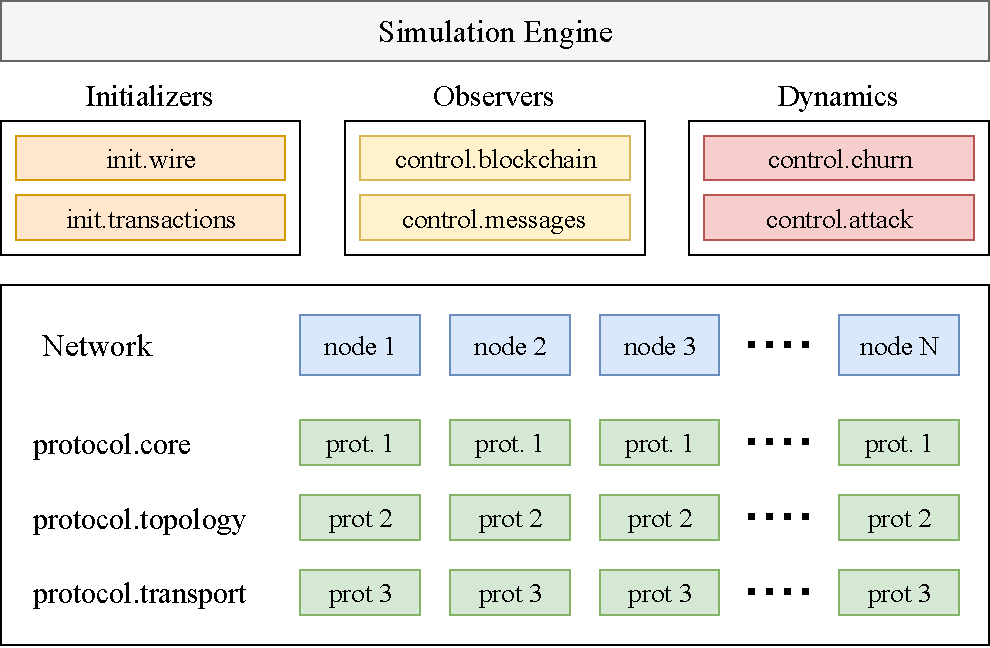
\includegraphics[scale=0.85]{figures/peersim}
	\vspace*{0.25cm}
	\caption[Illustration of the main components of a PeerSim simulation]{Illustration of the main components of a PeerSim simulation.}
	\label{fig:peersim}
\end{figure}

\subsubsection{EDSimulator}
The \texttt{EDSimulator} is a static singleton that implements the event-driven simulator engine.
It is the entry point of each simulation and it is responsible to manage its entire life-cycle:
load the configuration, bootstrap the network, run the initializers, keep the queue of events, schedule controls, and run the simulation loop.
It provides a method that can be used by any component to add new events to the queue.
The class is also able to run the same simulation multiple times using different seeds for the random number generators, in order to achieve a higher statistical significance.

\subsubsection{Event}
PeerSim does not have any class or interface to model an event.
Events are simply represented as plain Java objects, which are passed by reference to the simulator engine and to the target components.

\subsubsection{Network}
The \texttt{Network} class is a static singleton that keeps track of all nodes in the simulation.
Nodes are internally stored in an array and can be accessed by ID (their position in the array).
Information about neighbors of a node is stored in a special protocol \texttt{Linkable}.
It is used by all components that need to access a specific node or iterate over the available nodes.

\subsubsection{Node}
The network is composed of nodes.
A node is a container of protocols (each simulation can have \num{1} or more protocols).
The \texttt{Node} interface provides access to the protocols it holds, and to a fixed unique identifier of the node.
The behavior of a node is defined in each of the attached protocols.

\subsubsection{EDProtocol}
The \texttt{EDProtocol} interface defines a protocol that implements an event-driven behavior.
Protocols define the actions each node will perform during the simulation.
The interface has only the method \texttt{processEvent}, which is invoked by the scheduler to deliver events to the protocol.
Each node stores an array or protocols;
a class implementing this interface will have \num{1} instance for each node in the network.
Protocols can be stacked on each other to build more and more complex behaviors:
for example, an implementation of \texttt{EDProtocol} might be responsible to build and maintain a topology, while a second implementation may simulate some higher level functions, such as broadcasting some objects to the entire network in a gossip style using the underlying topology.
The simulation settings are specified with a configuration file;
some settings can be overridden with command line parameters.

\subsubsection{Linkable}
The \texttt{Linkable} interface provides a service to other protocols to access a set of neighbor nodes.
The instances of the same linkable class define an overlay network:
each instance has a list neighbors nodes.
Links do not need to be symmetric:
in some cases it could make sense to work with a directed graph.
The \texttt{Linkable} interface is usually implemented by protocols that exchanges messages over the network to build a topology.

\subsubsection{Transport}
The \texttt{Transport} interface models a transport layer in the OSI model \cite{wikipedia_osi}:
it is used to send messages through the underlying network.
Implementations of the \texttt{Transport} interface use the \texttt{EDSimulator} class to schedule the delivery of messages with some appropriate delay.
They can also model packet loss of packets and other failures.
Different transports can be stack on top of each other to model complex behaviors of the network.

\subsubsection{Control}
Classes implementing \texttt{Control} are used to define operations that require global network knowledge and management.
They can be scheduled for execution at certain points during the simulation, depending on their function.

\paragraph{Initializers}
Initializers are executed at the beginning of the simulation and are used to bootstrap the simulation.
Examples include creating the initial network topology, set the initial nodes' states and schedule the first events.

\paragraph{Dynamics}
Dynamics are executed periodically during the simulation and are used to modify the simulation in some way.
Examples include adding or removing nodes, creating a failure on the network, and introducing an extra delay for messages.

\paragraph{Observers}
Similar to dynamics, observers are executed periodically during the simulation.
They are used to read aggregated valued from nodes, and compute and collect statistics and metrics.

\subsubsection{Configuration}
\texttt{Configuration} is a static singleton class that provides access to the configuration for the current simulation.
It proxies all accesses to the configuration file and it allows to plug different strategies to load the configuration.
The configuration is stored as \texttt{<name, value>} pairs.
The class provides helper methods to perform common operations, such as reading values with type checking, resolving protocols by name, parsing mathematical expressions (that can be used in the configuration file), and resolving under-specified class-names.

\subsubsection{CommonState}
\texttt{CommonState} is a singleton static class that stores the state common to all components in the simulation.
Its main purposes is to simplify the simulator structure and increase the efficiency by avoiding some parameters passing.
It provides access to an instance of a pseudorandom number generator, already initialized with the provided seed and ready for use:
all components should use this instance to guarantee reproducibility of results.
Also, it stores the current time of the simulation.

\subsubsection{RangeSimulator}
The \texttt{RangeSimulator} is a utility class able to run simulations with ranges of parameters specified in the configuration file.
A range is a collection of values to be assigned to a variable.
If multiple ranges are specified, the class runs a simulation for all the possible combinations of values.
\texttt{RangeSimulator} invokes the standard PeerSim simulator engine to run each single experiment.

\subsection{Additional components}
In addition to the default PeerSim components, we developed the following new utilities.

\subsubsection{ParallelSimulator}
The \texttt{ParallelSimulator} is a utility class able to handle ranges and generate the list of their combinations:
parameters are read from the configuration file using the standard PeerSim mechanisms;
the class computes their combination and print them a list of commands, ready to be executed from the command line.
This class is particular useful when combined with the GNU Parallel, a shell tool for executing jobs in parallel using one or more computers \cite{gnu_parallel}.
Discrete event driven simulations are very difficult to parallelize, since events have causal relationships which are usually not well known in advance and are influenced by random variables:
in other words, they run on a single core do not exploit modern multi-core \ac{CPU}s.
To reduce the total completion time of a simulation with range parameters, one can use \texttt{ParallelSimulator} to generate the list of jobs to execute, then take advantage of GNU Parallel to run them in parallel.

\subsection{Simulation life cycle}
Each PeerSim simulation has the following life cycle:
\begin{itemize}
	\item load and validate the configuration; the configuration file defines which components are used and how they interact;
	\item run the initializers, in the order provided in the configuration file;
	\item schedule dynamics and observers, according to the parameters specified in the configuration;
	\item start the simulation loop and process one event at a time, until the maximum simulation time is reached, the queue of events is empty or some control terminates the simulation;
	\item run the controls scheduled for execution after the simulation;
	\item cleanup and schedule the next repetition of the experiment.
\end{itemize}

\section{Simulator design}

\subsection{Simplifications}

\subsection{Code structure}

\subsection{Metrics}


\printbibliography

\end{document}
